\section{问题设定}

令 $\tau \in [0,1]$ 通过错误率参数化裁判可靠度（judge reliability）：每次二元裁决（verdict）
以概率 $p = (1-\tau)/2$ 被翻转，因此 $\tau = 1$ 是完美裁判，$\tau = 0$ 相当于抛硬币。
令 $V \in [0,1]$ 表示生成器有效性（generator validity）：生成的任务中通过形式化验证器的比例。
令 $\Delta_t$ 表示第 $t$ 轮（round）的评估偏差（evaluation bias）：系统自评正确性与真值之间的
差距。

$\Delta_t^{\max}$ 是一个\emph{设计输入}，不是测量量：它是部署方愿意接受的端到端失败率上限，
在系统建成之前就已确定，并由第 5 节反解成所要求的裁判可靠度。下文实验是\emph{对照}它来读的，
而不是用来估计它；其可用区间不到二分之一。

\textbf{定义 1（安全区，safe zone）。} 若裁判可靠度
$\tau \ge \tau_c$ 且生成器有效性 $V \ge V_c$，则自进化智能体（self-evolving agent）处于安全区，
其中 $\tau_c$ 是把评估偏差控制在 $\Delta_t^{\max}$ 及以下所需的最低裁判可靠度（第 5 节），
$V_c = 0.5$ 是全文采用的生成器有效性下限。

表~\ref{tab:notation} 汇总了这套记号。

\begin{table*}[t]
  \centering
  \caption{记号表。第 3、4 节已在正文中逐条定义；最后两条仅在附录中使用。}
  \label{tab:notation}
  \small
  \begin{tabularx}{\textwidth}{@{}lX@{}}
    \toprule
    符号 & 含义 \\
    \midrule
    $\tau \in [0,1]$ & 裁判可靠度；每次裁决以概率 $p = (1-\tau)/2$ 被翻转。 \\
    $\tau_c$ & 临界 $\tau$：把评估偏差控制在 $\Delta_t^{\max}$ 及以下（第 5 节）。 \\
    $p$ & 单次裁决的翻转概率，$p = (1-\tau)/2$。 \\
    $V \in [0,1]$ & 生成器有效性：通过验证器的任务占比。 \\
    $V_c$ & 生成器有效性下限，$0.5$。 \\
    $\Delta_t$ & 第 $t$ 轮的评估偏差。 \\
    \midrule
    $\Delta_t^{\mathrm{gen}}$ & 生成侧失败率，$= 1 - V$。 \\
    $\Delta_t^{\mathrm{valid}}$ & 裁判侧失败率，以任务有效为条件。 \\
    $\Delta_t^{\mathrm{global}}$ & 端到端失败率，每个无效轮记 $\Delta_t = 1.0$。 \\
    $\Delta_t^{\max}$ & 设计输入：部署方愿意接受的端到端失败率上限。 \\
    $\Delta_{\mathrm{judge}}^{\mathrm{budget}}$ & 扣除 $\Delta_t^{\mathrm{gen}}$ 后留给裁判噪声的额度。 \\
    $n$ & 某个条件的轮数。 \\
    \midrule
    $S, G, J$ & 指示变量（附录~B）：成功、有效任务、判定正确。 \\
    $y, y^{*}$ & 提交的答案及其真值标签（附录~C）。 \\
    \bottomrule
  \end{tabularx}
\end{table*}

\textbf{命题 1（两个条件的必要性）。} 若 $\tau < \tau_c$，系统会累积
被污染的经验，且 $\Delta_t$ 单调增长。若 $V < V_c$，系统生成的大多是
无效任务，有效演化速率趋于零。

在 DeepSeek V4 Flash（\texttt{deepseek-flash}）上运行了 4 个条件 (A/B/C/D) $\times$ 200 轮 $\times$ 3 次运行 = 2400 轮。
主要指标为 $\Delta_t$；次要指标为有效任务率（valid task rate）。

\textbf{难度等级。} 等级是写进教师 prompt 的一个\emph{请求}，而不是工具链强制的属性：
L1 是线性整数算术（$\le$10 个变量），L2 是位向量（$\le$20），L3 混合 LIA、位向量与数组
（$\le$30），分别要求 3--5、3--8、3--10 条约束，求解器超时在 L1 为 5\,s、在 L2/L3 为 15\,s。
代码里只检查一个变量、一条约束与约束数不超过 50，因此等级只是一种\emph{意图}。它在
2{,}400 轮基线中是\emph{自适应}的（连续五轮判定正确且滑窗成功率 $\ge 0.8$ 时升级，
跌破 $0.3$ 时降级），而在 240 轮验证中是\emph{固定因子}，这正是只有后者的分级有效率可解释的原因。

% ===========================================================================
% 4. 双重瓶颈框架
% ===========================================================================
\section{双重瓶颈框架}

各条件（condition）的区别在于启用了哪些架构机制：A 既不启用形式化锚定（formal anchoring），也不启用
种群博弈（population game）；B 仅启用 Z3 形式化锚定；C 仅启用种群博弈；D 启用全部
机制（锚定 + 种群 + 蒸馏（distillation） + 圆桌共识（round-table consensus））。无效轮——即
教师（teacher）未能产出可求解的约束集（constraint set）的那些轮——在 \textit{global} 口径下被编码为 $\Delta_t = 1.0$，
而在 \textit{valid-only} 口径下被排除。
图~\ref{fig:bottleneck_and_validity} 并排展示了这两个瓶颈。

\subsection{合成律}

当评估信号未被形式化锚定时，裁判一侧的瓶颈就会出现：
系统的自评会偏离真值，且这种偏离会不断累积。生成器一侧的
瓶颈则在难度控制器（difficulty controller）超出教师编写良构
实例的能力时出现。系统只有在两个安全区的交集之内才是安全的：裁判
可靠度 $\tau \ge \tau_c$ \textbf{且}生成器有效任务率 $\ge 0.5$。在这一交集之外，
系统仍然会产出日志，仍然会在它能完成的那些轮上报告成功，也仍然
看起来在运行——这正是该失效容易被忽视的原因。

第二个瓶颈背后的直觉是：因果变量并不是 $\tau_c$ 本身。记 $\Delta_t^{\mathrm{gen}}$ 为
\textbf{生成侧失败率}——教师未能产出形式化校验器可接受任务的轮次占比，因此
$1 - \Delta_t^{\mathrm{gen}}$ 就是第 3 节的有效任务率 $V$；记 $\Delta_t^{\mathrm{valid}}$ 为
\textbf{以任务有效为条件的裁判侧失败率}，其分母只计有效轮次，因为无效任务根本没有可供评判的
答案；$\Delta_t^{\mathrm{global}}$ 则是\textbf{端到端失败率}，对全部轮次统计，每个无效轮记
$\Delta_t = 1.0$。一轮只有在有效任务存在 \textit{且}学生（student）的答案被判正确时才算成功，
因此两个失败率按链式法则（chain rule）合成：

\[
  1 - \Delta_t^{\mathrm{global}} = (1 - \Delta_t^{\mathrm{gen}})(1 - \Delta_t^{\mathrm{valid}})
\]

这个式子的读法是一条关于分母的陈述：有效轮次上的成功率，被"产出可用任务的轮次占比"
重新标定。在 2400 轮数据上，该式成立至机器精度（machine precision）（附录~D，表~\ref{tab:table4c_appendix}）。

\begin{figure}[t]
  \centering
  \begin{minipage}{0.48\linewidth}
    \centering
    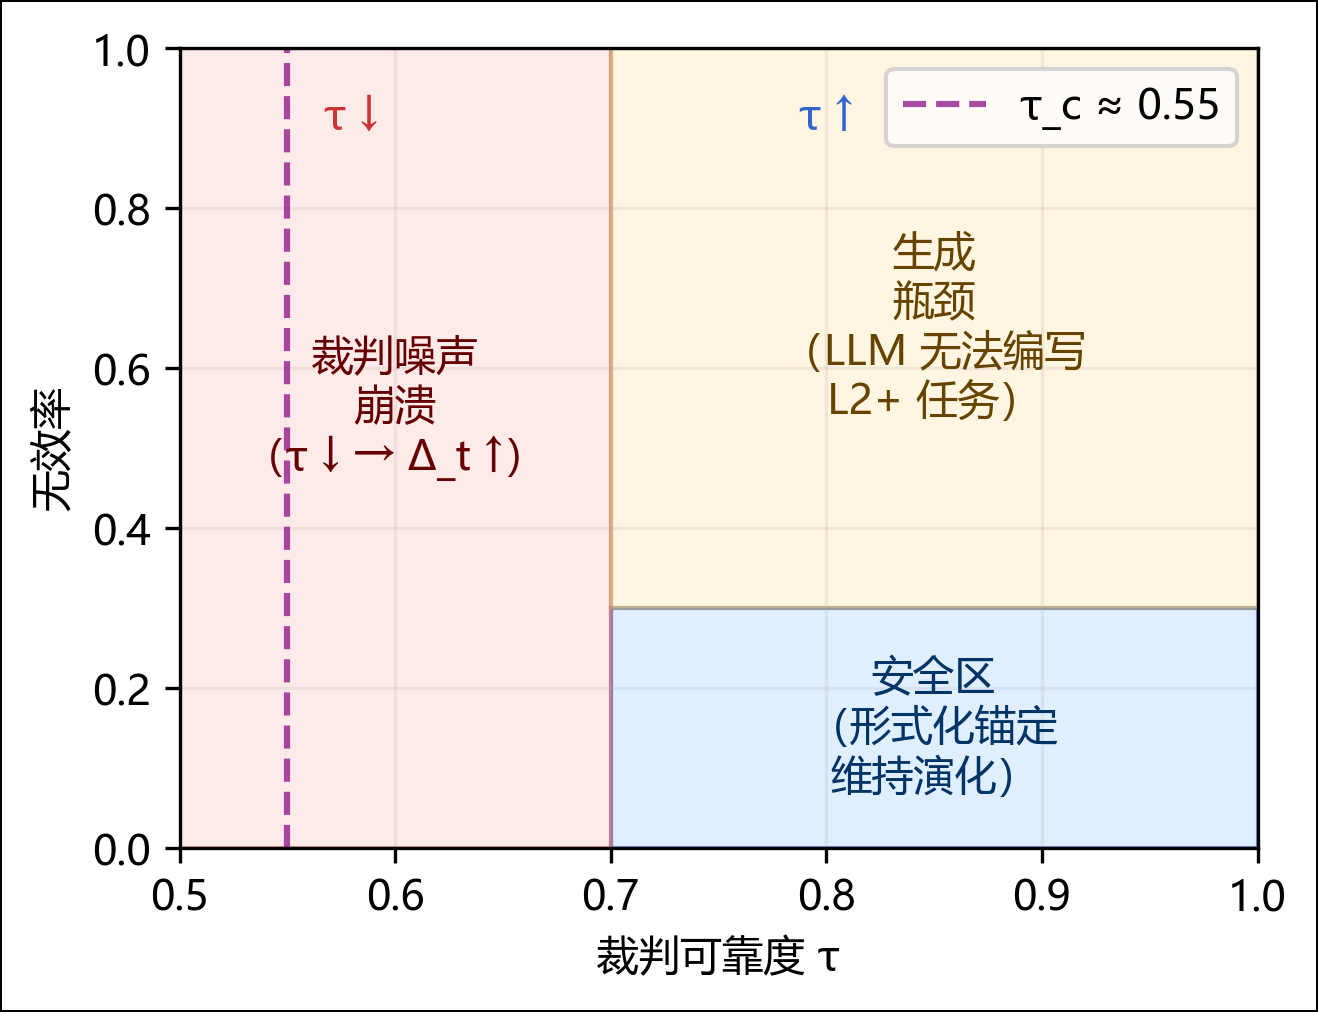
\includegraphics[width=\linewidth]{figures_zh/fig1_dual_bottleneck.png}
  \end{minipage}\hfill
  \begin{minipage}{0.48\linewidth}
    \centering
    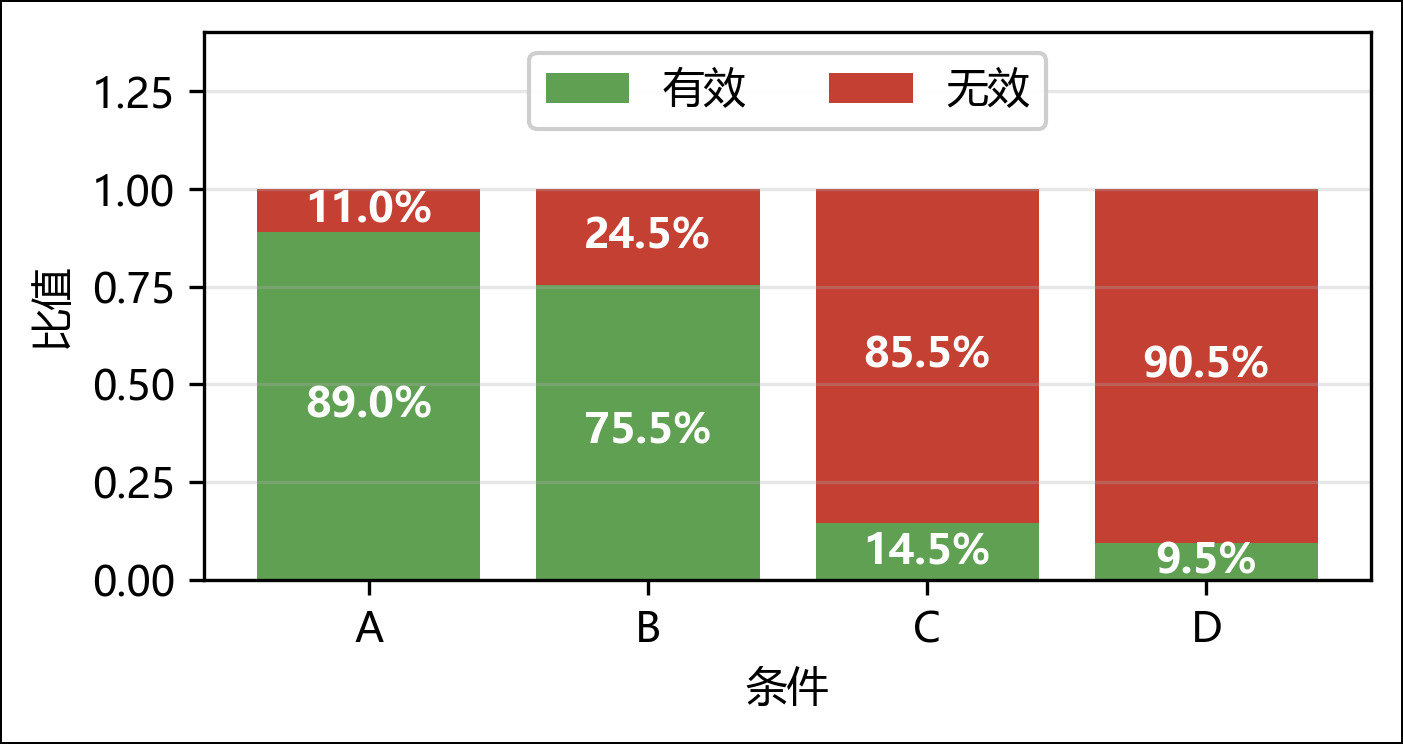
\includegraphics[width=\linewidth]{figures_zh/fig3_validity_rate.png}
  \end{minipage}
  \caption{左图：安全区即裁判可靠度
  $\tau \ge \tau_c$ 与生成器无效任务率 $\le 0.5$ 的交集。右图：有效任务
  率从 89.0\%（A）和 75.5\%（B）跌至 14.5\%（C）和 9.5\%（D）。}
  \label{fig:bottleneck_and_validity}
\end{figure}

\subsection{两个瓶颈}

在 valid-only 口径下，条件 A（LLM 自评分）给出 $\Delta_t = 0.150$，条件 B
（Z3 锚定）给出 $0.000$：只要任务是良构的，锚定的裁决 \textit{就是}真值，
因此自评分偏离在构造上即消失。在 global 口径下，同样的条件读作
A = 0.243、B = 0.245，因为 B 的 147 个无效轮被计入 $\Delta_t = 1.0$。这是
口径差异，而非数据不一致；见附录~\ref{app:data_consistency} 与
图~\ref{fig:bottleneck_and_validity}。

裁判并不是唯一的瓶颈。一旦启用种群博弈（C 与 D），控制器
会把任务推向 L2/L3，而教师无法可靠地编写位向量与数组约束：
有效率从 89.0\%（A）和 75.5\%（B）跌至 14.5\%（C）和 9.5\%（D）。这些失败
\textit{并非}按难度分级——它们聚集在过渡处，因为控制器一直把难度维持在
高位，而教师持续失败。称之为\textbf{伪难度陷阱}（pseudo-difficulty trap）：
系统自以为在解决更难的问题，实际上却把预算花在了永远无法进入
验证环节的任务上。学生并没有过错；每一个含有有效任务的轮都被正确解决
（图~\ref{fig:bottleneck_and_validity}）。

\subsection{预算分解}

因此，这两个瓶颈\textbf{共享同一份预算}。给定可容忍的 global 误差
$\Delta_t^{\max}$，留给裁判噪声的额度为

\[
  \Delta_{\mathrm{judge}}^{\mathrm{budget}} = 1 - \frac{1-\Delta_t^{\max}}{1-\Delta_t^{\mathrm{gen}}}
  \qquad\Longrightarrow\qquad
  \tau_c = \sqrt{1 - 2\,\Delta_{\mathrm{judge}}^{\mathrm{budget}}}
\]

因此，$\tau_c$ 并不是某个条件的机制所固有的属性——它是
\textbf{推导}出来的，取决于生成器瓶颈在预算中剩下多少。一个
$\Delta_t^{\mathrm{gen}}$ 较大的条件，在相同的总容忍度下需要更可靠的裁判，但真正的驱动因素是
预算的分配，而不是 $\tau_c$ 本身。

具体地，在 $\Delta_t^{\max} = 0.60$ 时：条件 B（$\Delta_t^{\mathrm{gen}} = 0.245$）需要
$\tau_c \approx 0.24$，而 C 与 D（$\Delta_t^{\mathrm{gen}} = 0.855$ 和 $0.905$）在
\textbf{任何}裁判可靠度下都无法满足该预算，因为它们的生成器瓶颈本身就已超出
预算。这才是预算直觉的正确形式，它把双重瓶颈（dual bottleneck）框架从一种
诊断转变为一条核算规则。

% ===========================================================================
% 5. 裁判可靠度阈值
% ===========================================================================
\section{裁判可靠度阈值}
\label{sec:judge}

本节只问一个问题：给定一个能够产生候选改进的生成器，裁判必须多可靠，迭代式自我改进才能带来净收益？分四步回答。\S\ref{sec:noise} 定义了把裁判可靠度参数化的噪声注入（noise injection）协议。\S\ref{sec:empirical_tau} 在真实智能体轨迹上估计经验阈值 $\tau_c$。\S\ref{sec:analytical} 从合成律（composition law）出发推导 $\tau_c$ 的闭式表达式。\S\ref{sec:theorem1} 陈述并证明由此得到的可靠度定理。

\subsection{噪声注入协议}
\label{sec:noise}

通过对每个裁决以概率 $p = (1-\tau)/2$ 进行翻转来建模不可靠的裁判，
对 SAT 与 UNSAT 对称处理。每一轮有两个独立的 Z3 调用被注入噪声——
即对教师任务的裁决和对学生答案的裁决——因此它们独立地翻转。

\subsection{经验 $\tau_c$}
\label{sec:empirical_tau}

在条件 B 与 D 上把 $\tau$ 扫过八个取值 $\{0.55, 0.60, 0.65, 0.70, 0.75, 0.80, 0.90, 1.00\}$，
每个格子（cell）50 轮（共 800 轮），使用 \textbf{真实的} DeepSeek V4
Flash API。所有轮都被固定在难度 L1，以使生成器一侧的瓶颈保持
不变，只有裁判的可靠度发生变化。经验曲线见附录~A，
图~\ref{fig:tau_c_curve_appendix}。

一次先导性估计曾给出 $\tau_c(D) = 0.90$ 与 $\tau_c(B) = 0.55$。
该差距在 L1 隔离下未能复现：固定难度恰好移除了该假设所诉诸的机制。

在八个被扫描的 $\tau$ 取值上，条件 B 实测的逐格子均值 $\Delta_t$ 从
$\tau = 0.55$ 时的 0.30 下降到 $\tau = 1.00$ 时的 0.00。其形状是开口
向下的抛物线，而非直线，并且它在 $\tau = 0$ 处穿过 0.5，而不是穿过 1.0。这两个
特征最终都被证明对该机制具有诊断意义，如第~5.3~节所示。检测到的阈值为
在所有三种口径（combined、$\Delta_t$、correct-rate）下 $\tau_c(B) = \tau_c(D) = 0.55$。

\subsection{解析公式}
\label{sec:analytical}

\textbf{假设 1（裁判噪声）。} 每个 Z3 裁决都被独立翻转，其概率为

\[
  p = \frac{1-\tau}{2}
\]

\textbf{假设 2（每轮两次独立判定）。} 一轮涉及两次彼此独立的 Z3 调用：
一次产出对教师任务的裁决（该结果成为 \texttt{expected}），另一次产出
对学生答案的裁决。它们是彼此分离的进程，并且独立地翻转。

当且仅当两个裁决\textbf{一致}时——即都未被翻转，或都被
翻转时——该轮才被记为正确：

\[
  P(\text{correct}) = (1-p)^2 + p^2
\]

代入 $p = (1-\tau)/2$，从而 $1-p = (1+\tau)/2$：

\[
  P(\text{correct}) = \left(\frac{1+\tau}{2}\right)^2 + \left(\frac{1-\tau}{2}\right)^2
  = \frac{(1+\tau)^2 + (1-\tau)^2}{4} = \frac{2 + 2\tau^2}{4} = \frac{1+\tau^2}{2}
\]

因此

\[
  \boxed{\;\Delta_t(\tau) = 1 - P(\text{correct}) = \frac{1-\tau^2}{2}\;}
\]

\textbf{$\tau^2$ 与 $1/2$ 从何而来。} $\tau^2$ 是两个一致项之和——
都正确贡献 $((1+\tau)/2)^2$，都被翻转贡献 $((1-\tau)/2)^2$——
它们的交叉项相互抵消，剩下 $(1+\tau^2)/2$；因此该指数是每轮独立
判定的次数，而不是裁判自身的属性。$1/2$ 来自 SAT/UNSAT 的二元对称性：在
$\tau = 0$ 时，两个独立的随机裁决有一半的时间一致，这就是曲线左端为何锚定在
0.5 而不是 1.0。

在八个被扫描的 $\tau$ 取值上，实测的逐格子均值与闭式解吻合，具体为

\begin{itemize}
  \item MAE = \textbf{0.0258}，RMSE = 0.0329（条件 B）
  \item MAE = \textbf{0.0520}，RMSE = 0.0660（条件 D）
\end{itemize}

\textbf{一个具有判别力的检验。} 假设 2 中的机制并不是唯一能给出
相同 $\Delta_t(\tau)$ 的解释。另一种解释——裁判以概率 $\tau$ 判断正确
\textit{且}系统以概率 $\tau$ 接受该判断——预测
$P(\text{correct}) = \tau^2$，而非 $(1+\tau^2)/2$。两者差异悬殊，因此实测的
\texttt{correct\_rate} 无需任何拟合即可区分它们：

\begin{center}
\small
\begin{tabular}{@{}llr@{}}
  \toprule
  模型 & $P(\text{correct})$ & 相对实测 \texttt{correct\_rate} 的 MAE \\
  \midrule
  两次独立判定（\textbf{本工作}） & $(1 + \tau^2)/2$ & \textbf{0.0389} \\
  裁判 + 接受 & $\tau^2$ & 0.2291 \\
  \bottomrule
\end{tabular}
\end{center}

在 16 个 $(\tau, \text{condition})$ 格子中，两次判定模型在 13 个上更接近、在 2 个上持平，
在 1 个上落败。在 $\tau = 0.80$ / 条件 B 处，它预测 0.8200，而实测为 0.8200。
接受假说在 MAE 上以六倍的差距被拒绝。

\textbf{反解模型。} 由 $\Delta_t = (1 - \tau^2)/2$ 解出 $\tau$，得到设计规则

\[
  \tau_c = \sqrt{1 - 2\,\Delta_t^{\max}}
\]

因此，一个能够容忍误差下界 $\Delta_t^{\max}$ 的系统，需要可靠度至少达到该值的
裁判：

\begin{center}
\small
\begin{tabular}{@{}rr@{}}
  \toprule
  $\Delta_t$ 预算 & 所需的 $\tau_c$ \\
  \midrule
  0.05 & 0.949 \\
  0.10 & 0.894 \\
  0.15 & 0.837 \\
  0.20 & 0.775 \\
  0.25 & 0.707 \\
  \bottomrule
\end{tabular}
\end{center}

这是该结果在实践中有用的形式：它把对评估误差的容忍度转换为
对裁判的最低可靠度要求，而无需重新运行扫描。请注意
可达性上界——没有任何裁判可靠度能把 $\Delta_t$ 保持在 0.5 以下，因为 $\Delta_t(0) = 1/2$。
解析拟合已叠加显示在附录~A、图~\ref{fig:analytical_fit_appendix} 中。

\subsection{定理 1：裁判可靠度阈值}
\label{sec:theorem1}

在第~5.3~节所述的假设下，以定理的形式陈述该阈值。
图~\ref{fig:theorem1} 展示了该阈值。

\textbf{定理 1。} \textit{系统的期望评估偏差为}

\[
  \Delta_t(\tau) \;=\; \frac{1-\tau^{2}}{2}
\]

\textit{不含自由参数；等价地，$P(\text{correct}) = (1+\tau^{2})/2$，且
$\Delta_t(0) = 1/2$。}

\textbf{逆向（设计）形式。} 解出 $\tau$ 可得在可容忍偏差 $\Delta_t^{\max}$ 下
最小的可接受裁判可靠度：

\[
  \tau_c \;=\; \sqrt{1 - 2\,\Delta_t^{\max}}
\]

由于 $\Delta_t(0) = 1/2$，没有任何裁判可靠度能把偏差保持在 $1/2$ 以下，因此该规则
仅在 $\Delta_t^{\max} \in [0, 1/2)$ 上有定义。

\textbf{推论（裁判稀缺性）。} $\tau_c$ 是可容忍偏差的函数，\textbf{而}不是
系统的常数。在 $\Delta_t^{\max} = 0.35$ 时，一个大约每五次裁决错一次的裁判
（$\tau \approx 0.55$）仍能使系统保持在安全区内；把容忍度收紧到
$0.05$ 则需要 $\tau \approx 0.95$。

\textbf{经验验证。} 在 800 个真实 API 轮上拟合（8 个 $\tau$ 取值 $\times$ 2
个条件 $\times$ 50 轮，难度固定为 L1）：MAE = \textbf{0.0258} / RMSE = 0.0329（B）
以及 MAE = \textbf{0.0520} / RMSE = 0.0660（D）。

\textbf{注记（被拒绝的替代模型）。} 一个竞争模型——裁判以概率 $\tau$ 判断正确
\textit{且}系统以概率 $\tau$ 接受该判断——预测
$P(\text{correct}) = \tau^{2}$，因而 $\Delta_t = 1-\tau^{2}$。判别检验\textbf{无需任何拟合}
即可拒绝它：相对于实测 \texttt{correct\_rate} 的 MAE 为 0.2291，而
定理 1 为 0.0389；在 16 个格子中定理 1 于 13 个上更接近、2 个持平、1 个落败。在
$\tau = 0.55$ 处，它预测 0.6975，而实测为 0.3000（B）和 0.3200（D）。本文没有任何结果
使用 $\Delta_t = 1-\tau^{2}$。

\textbf{与 Ratchet 界的关系。} Ratchet 的分析给出 $(1 - \tau)/2$，作为
\textbf{单次}判定被翻转的概率。量是\textbf{双次}判定
系统的稳态误差。两者通过一致概率相联系，而这种
区别是结构性的，而非数值上的：

\begin{center}
\small
\begin{tabular}{@{}lll@{}}
  \toprule
  设定 & 每次决策中的噪声事件 & 误差 \\
  \midrule
  技能消除（Ratchet） & 一次判定，然后据此行动 & $(1 - \tau)/2$ \\
  答案评估（本工作） & 裁判的裁决\textbf{与}系统的裁决必须一致 & $(1 - \tau^2)/2$ \\
  \bottomrule
\end{tabular}
\end{center}

两者之间的映射是两次判定中恰好只有一次被翻转的概率：

\[
  \Delta_t = 2p(1-p) \;\xrightarrow{p \to 0}\; 2p = 1-\tau
\]

因此，在高可靠度极限下两者在一阶上一致，而离开该极限后则以二次方式
分岔。在 $\tau = 0.95$ 时，单次判定界预测 0.025，而双次判定模型
预测 0.049：在该可靠度下，要求两个独立裁决一致会使可容忍误差
减半。Ratchet 的界是系统仅依据一次判定行动时的特例；
此处的公式把它推广到依据两次判定之间的一致性行动的系统。

\begin{figure*}[t]
  \centering
  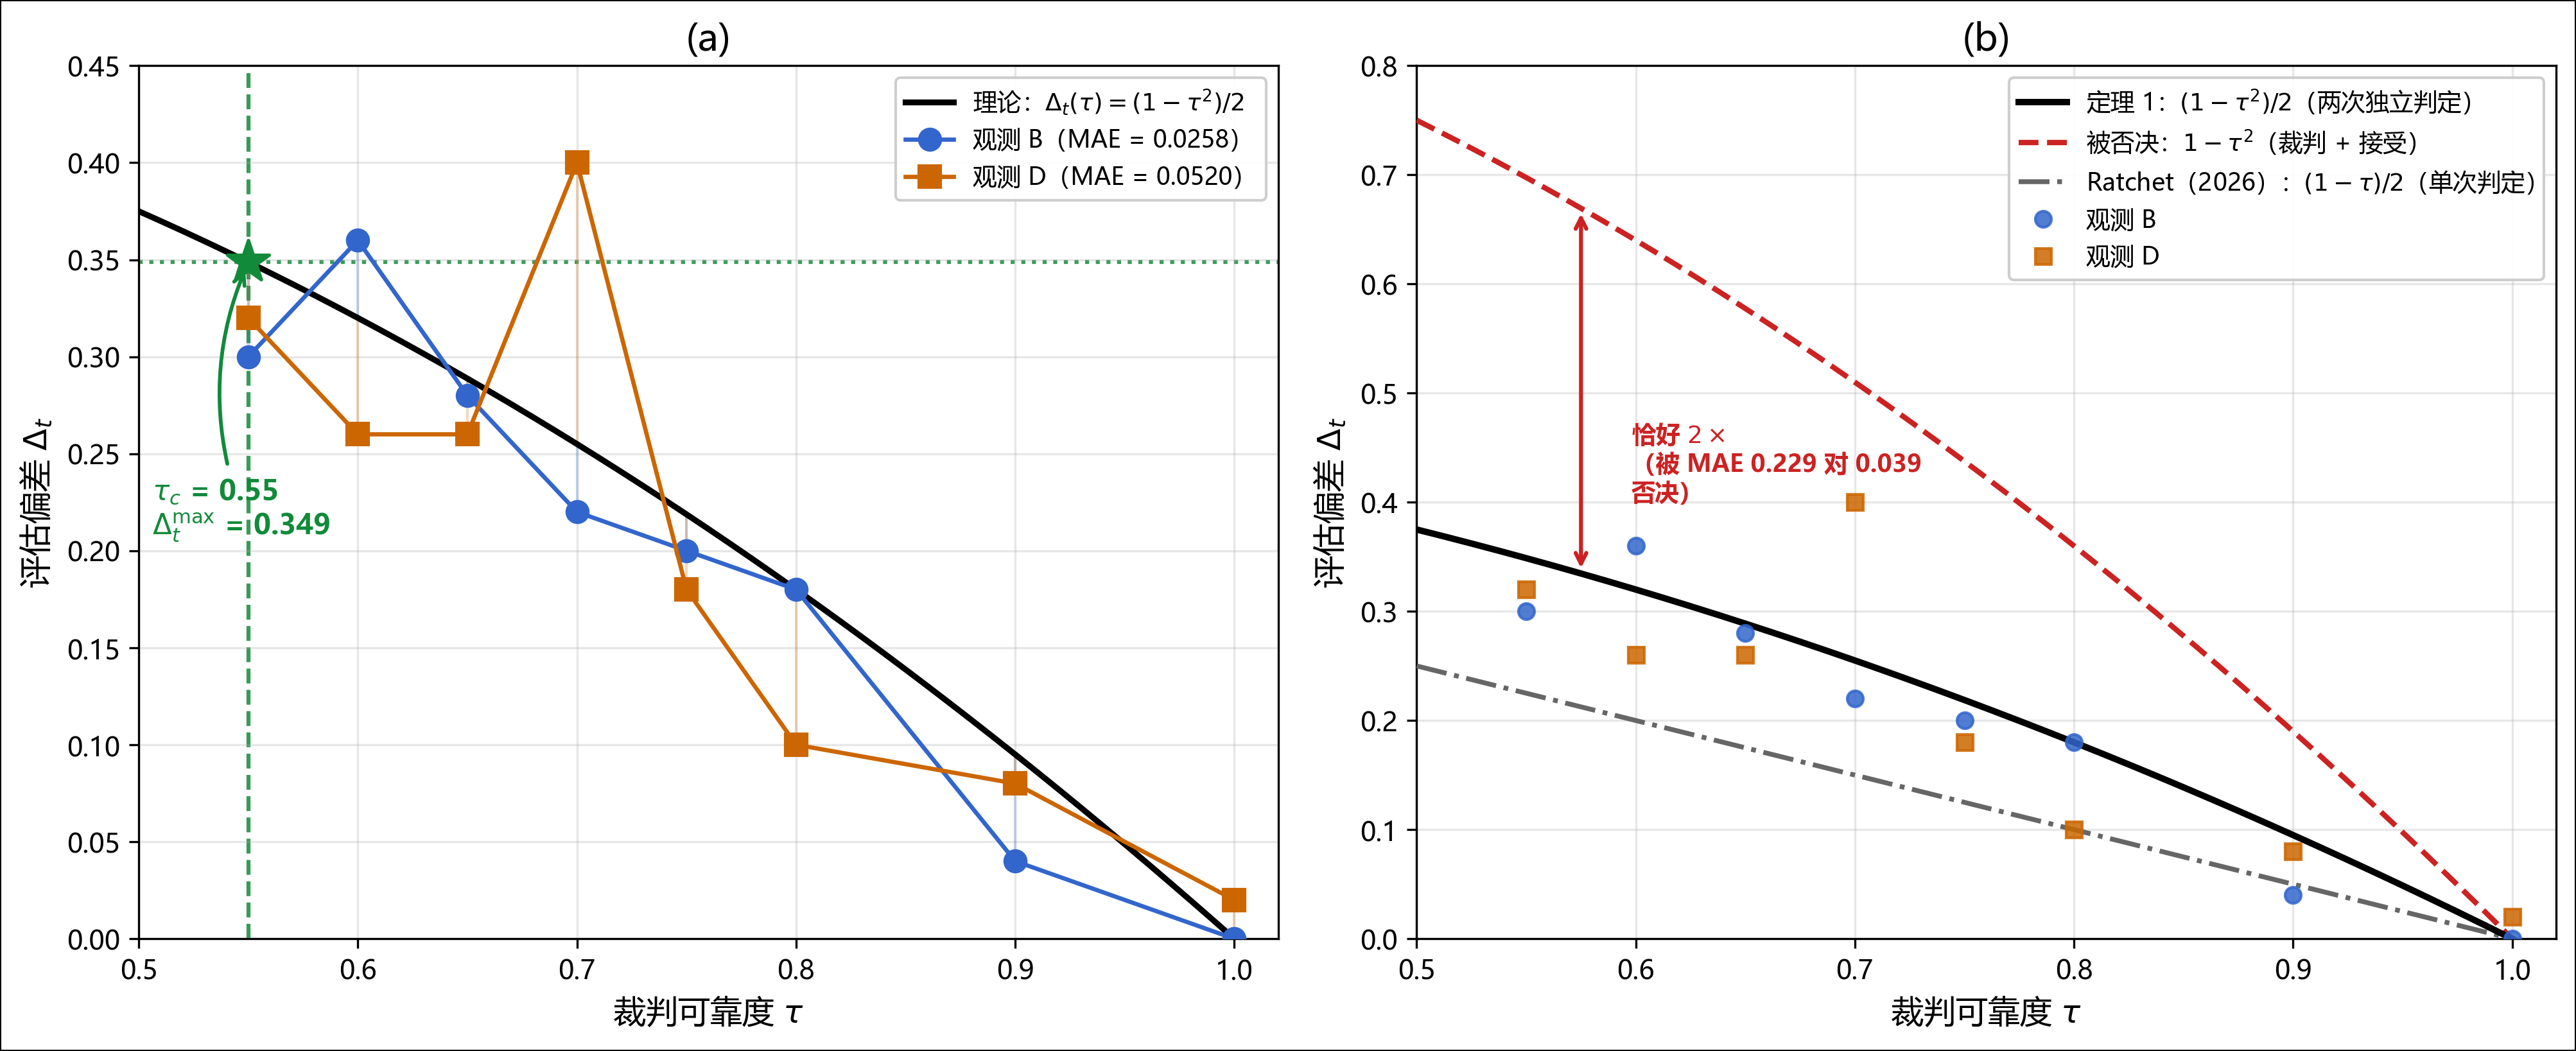
\includegraphics[width=\textwidth]{figures_zh/fig5c_theorem1.png}
  \caption{子图 (a)：闭式解 $\Delta_t(\tau) = (1-\tau^2)/2$ 与条件 B 和 D 的真实 API 扫描
  的对比，其中标出了实测的 $\tau_c = 0.55$ 及相应的
  $\Delta_t^{\max} = 0.349$。子图 (b)：同一闭式解与被拒绝的接受
  模型（$\Delta_t = 1-\tau^2$）以及 Ratchet 的单次判定界（$(1-\tau)/2$）的对比；接受
  模型恰好高出两倍，并被第~5.3~节的判别检验所拒绝。}
  \label{fig:theorem1}
\end{figure*}

% ===========================================================================
% 6. 扩展生成器能力
% ===========================================================================
